
\documentclass{report}

\usepackage[utf8]{inputenc}
\usepackage[italian]{babel}
\usepackage{import}
\usepackage{todonotes}
\usepackage{color}
\usepackage{rotating}
\usepackage[hidelinks]{hyperref}
\usepackage{url}
\usepackage{pdfpages}
\usepackage{siunitx}
\usepackage{pdflscape}
\usepackage{subfig}
\usepackage[euler]{textgreek}
\usepackage{mhchem}

\usepackage{enumerate} 
\usepackage{amsmath}
\usepackage{amsfonts}

\usepackage[signatures,swapnames,sans]{frontespizio}

\usepackage{geometry}
\geometry{portrait, margin=3cm}
\usepackage{siunitx}
\usepackage{booktabs}

\renewcommand*\figurename{Figura}

\newcommand{\sub}[1]{\textsubscript{#1}}
\newcommand{\super}[1]{\textsuperscript{#1}}
\newcommand{\parallelsum}{\mathbin{\!/\mkern-5mu/\!}}

\newcommand{\Fig}[0]{Fig.}

\usepackage{titlesec}

\titleformat{\chapter}{\normalfont\huge}{}{20pt}{\huge\bfseries}

\linespread{1.3}

\begin{document}
\addtocounter{chapter}{+5}
	\begin{frontespizio}
		\Margini{3cm}{3cm}{3cm}{3cm}
		\Universita{Bergamo}
		\Logo[43.332mm]{unibg-mark}
		\Divisione{Scuola di Ingegneria}
		\Corso[Laurea Magistrale]{Ingegneria Informatica}
		\Titolo{Laboratorio di Elettronica}
		\Sottotitolo{Relazione progetto circuito}
		\Punteggiatura{}
		\NRelatore{Prof.}{Prof.}
		\Relatore{Luigi Gaioni}
		\Candidato[1058231]{Giulia Allievi}
		\Candidato[1059640]{Martina Fanton}
		\Annoaccademico{2022--2023}
		\begin{Preambolo*}
			\usepackage[italian]{babel}
			\usepackage[T1]{fontenc}
			\usepackage[utf8]{inputenc}
			\usepackage{microtype}
			\usepackage{lmodern}
			\graphicspath{{img/}}
			
			\renewcommand{\frontinstitutionfont}{\fontsize{14}{17}\bfseries\scshape}
			\renewcommand{\fronttitlefont}{\fontsize{17}{21}\bfseries\scshape}
			\renewcommand{\frontfootfont}{\fontsize{12}{14}\bfseries\scshape}
		\end{Preambolo*}
	\end{frontespizio}

%----------------------------------------------------------------------------------------
%	PAGINA BIANCA
%----------------------------------------------------------------------------------------
\newpage
\null
\thispagestyle{empty}
\newpage

\chapter{Relazione progetto circuito}
\section*{Introduzione}
Il progetto richiede di realizzare un circuito che, superata una temperatura di riferimento, generi un allarme luminoso lampeggiante. Il sistema deve essere automatico, reversibile e realizzato hardware, senza avere a disposizione microcontrollori. Si hanno a disposizione:
\begin{itemize}
\item un termistore NTC;
\item un LED rosso;
\item un comparatore;
\item un timer 555;
\item componenti passivi.
\end{itemize}
La temperatura di riferimento è \SI{25}{\degree C}, a questa temperatura la resistenza del termistore NTC è di \SI{1}{k\ohm}.

\newpage
\section{Progettazione del circuito}
Per progettare il circuito, progetteremo e dimensioneremo separatamente la rete del termistore e la rete oscilllante, quindi integreremo le sue sottoreti per ottenere il progetto del sistema finale.
\subsection{Progettazione della rete oscillante}
Inizialmente progettiamo la rete oscillante. Configuriamo il timer 555 in modo tale che funzioni in modalità astabile. Lo schema scelto è mostrato in figura \ref{figura:schema555}, i pin sono collegati in questo modo:
\begin{itemize}
\item PIN 1, è il terminale di \textit{ground}, perciò è collegato a massa;
\item PIN 2, è il terminale di \textit{trigger}, è cortocircuitato con il PIN 6;
\item PIN 3, è l'\textit{uscita}, qui sarà collegato il LED tramite una resistenza;
\item PIN 4, è il terminale di \textit{reset}, servirà per gestire il collegamento alla rete che gestisce il termistore;
\item PIN 5, è il terminale di \textit{control voltage}, non lo utilizziamo, è collegato a massa tramite una capacità di filtraggio ($\mathrm{C_1}$);
\item PIN 6, è il terminale di \textit{threshold}, gestisce la carica della capacità $\mathrm{C_2}$ attraverso la resistenza $\mathrm{R_1}$;
\item PIN 7, è il terminale di \textit{discharge}, pilota la scarica della capacità $\mathrm{C_2}$ attraverso la resistenza $\mathrm{R_2}$;
\item PIN 8, è il terminale di \textit{alimentazione}. 
\end{itemize} 
Tra i pin 6 e 7 viene collegato un diodo (l'anodo è collegato al pin 7 mentre il catodo al pin 6), la sua funzione è quella di bypassare la resistenza $\mathrm{R_2}$ nella fase di carica del condensatore, in modo tale da ottenere un oscillatore con duty cycle variabile da 0\% a 100\%. 
\begin{figure}[h!]
	\centering
	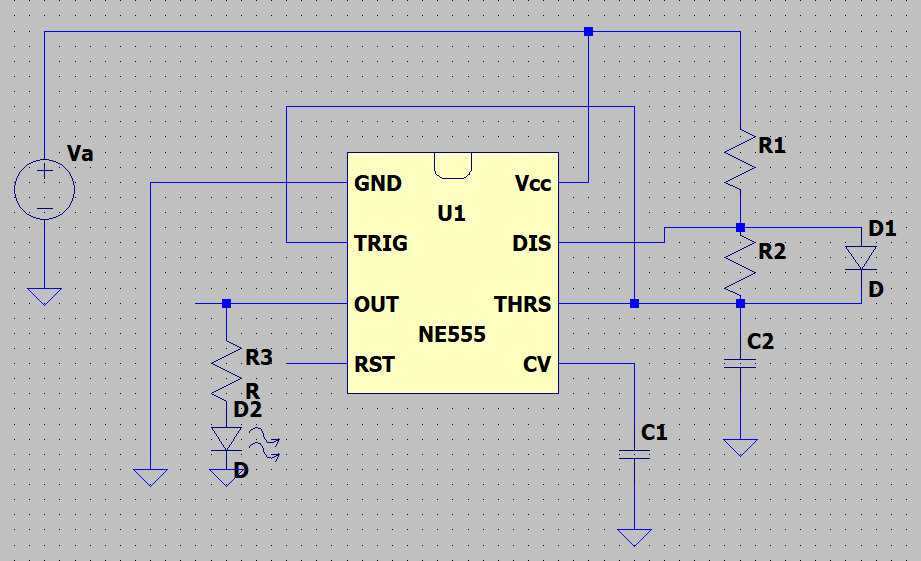
\includegraphics[height=6.5cm]{immagini/schema555}
	\caption{Schema della rete oscillante.} 
	\label{figura:schema555}
\end{figure}
\\Successivamente, dimensioniamo i passivi della rete oscillante.
\\va
\\cv
\\ led
\\ resto (rete oscillante vera e propria)

\subsection{Progettazione della rete del termistore}

\newpage
\section{Simulazione del circuito}
\subsection{Simulazione della rete oscillante}
\subsection{Simulazione della rete del termistore}



\end{document}